\documentclass[12pt, letterpaper]{report}
\usepackage[utf8]{inputenc}
\usepackage{tikz}

\title{Relazione Algoritmi e Strutture Dati}
\author{Eduard Antonovic Occhipinti, Iman Solaih, Marco Molica}

\begin{document}
\maketitle
\tableofcontents

\chapter*{Esercizio 1}
\section{Quick Sort}
Il \verb|quick_sort()| è un algoritmo che ordina una collezione partendo da un pivot, 
il pivot può essere scelto in vari modi, e in base a quale viene scelto il tempo
di sorting varia. Il \verb|quick_sort()| utilizza \verb|_part()| per scegliere il pivot prima 
di chiamare \verb|partition()| per dividere gli elementi del range selezionato 
in un sottoinsieme di elementi maggiori e uno di elementi minori del pivot
la cui posizione finale viene restituita dal metodo.

\subsection{Impatto della scelta del pivot nel quick sort}
La chiamata a \verb|rand()| porta il \verb|quick_sort()| con pivot scelto 
randomicamente o come mediana di tre numeri ad essere mediamente più lento 
rispetto agli altri 3 casi presi in considerazione. La tabella sottostante 
riporta il tempo impiegato ad ordinare un array di 20 milioni elementi di tipo \verb|struct Record|
% Created by tikzDevice version 0.12.3.1 on 2022-04-28 16:57:06
% !TEX encoding = UTF-8 Unicode
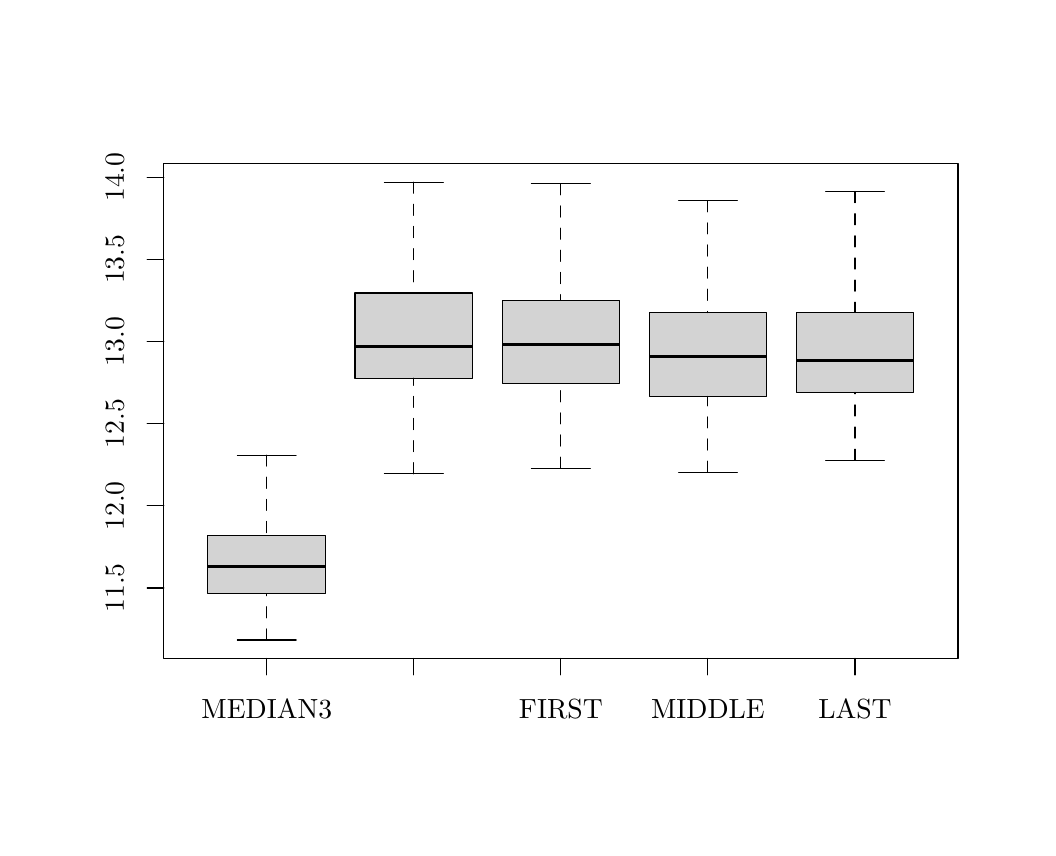
\begin{tikzpicture}[x=1pt,y=1pt]
\definecolor{fillColor}{RGB}{255,255,255}
\path[use as bounding box,fill=fillColor,fill opacity=0.00] (0,0) rectangle (361.35,289.08);
\begin{scope}
\path[clip] ( 49.20, 61.20) rectangle (336.15,239.88);
\definecolor{fillColor}{RGB}{211,211,211}

\path[fill=fillColor] ( 65.14, 84.58) --
	(107.65, 84.58) --
	(107.65,105.56) --
	( 65.14,105.56) --
	cycle;
\definecolor{drawColor}{RGB}{0,0,0}

\path[draw=drawColor,line width= 1.2pt,line join=round] ( 65.14, 94.31) -- (107.65, 94.31);

\path[draw=drawColor,line width= 0.4pt,dash pattern=on 4pt off 4pt ,line join=round,line cap=round] ( 86.40, 67.82) -- ( 86.40, 84.58);

\path[draw=drawColor,line width= 0.4pt,dash pattern=on 4pt off 4pt ,line join=round,line cap=round] ( 86.40,134.63) -- ( 86.40,105.56);

\path[draw=drawColor,line width= 0.4pt,line join=round,line cap=round] ( 75.77, 67.82) -- ( 97.02, 67.82);

\path[draw=drawColor,line width= 0.4pt,line join=round,line cap=round] ( 75.77,134.63) -- ( 97.02,134.63);

\path[draw=drawColor,line width= 0.4pt,line join=round,line cap=round] ( 65.14, 84.58) --
	(107.65, 84.58) --
	(107.65,105.56) --
	( 65.14,105.56) --
	cycle;

\path[fill=fillColor] (118.28,162.43) --
	(160.79,162.43) --
	(160.79,193.22) --
	(118.28,193.22) --
	cycle;

\path[draw=drawColor,line width= 1.2pt,line join=round] (118.28,173.97) -- (160.79,173.97);

\path[draw=drawColor,line width= 0.4pt,dash pattern=on 4pt off 4pt ,line join=round,line cap=round] (139.54,127.87) -- (139.54,162.43);

\path[draw=drawColor,line width= 0.4pt,dash pattern=on 4pt off 4pt ,line join=round,line cap=round] (139.54,233.26) -- (139.54,193.22);

\path[draw=drawColor,line width= 0.4pt,line join=round,line cap=round] (128.91,127.87) -- (150.16,127.87);

\path[draw=drawColor,line width= 0.4pt,line join=round,line cap=round] (128.91,233.26) -- (150.16,233.26);

\path[draw=drawColor,line width= 0.4pt,line join=round,line cap=round] (118.28,162.43) --
	(160.79,162.43) --
	(160.79,193.22) --
	(118.28,193.22) --
	cycle;

\path[fill=fillColor] (171.42,160.38) --
	(213.93,160.38) --
	(213.93,190.57) --
	(171.42,190.57) --
	cycle;

\path[draw=drawColor,line width= 1.2pt,line join=round] (171.42,174.68) -- (213.93,174.68);

\path[draw=drawColor,line width= 0.4pt,dash pattern=on 4pt off 4pt ,line join=round,line cap=round] (192.67,129.91) -- (192.67,160.38);

\path[draw=drawColor,line width= 0.4pt,dash pattern=on 4pt off 4pt ,line join=round,line cap=round] (192.67,232.64) -- (192.67,190.57);

\path[draw=drawColor,line width= 0.4pt,line join=round,line cap=round] (182.05,129.91) -- (203.30,129.91);

\path[draw=drawColor,line width= 0.4pt,line join=round,line cap=round] (182.05,232.64) -- (203.30,232.64);

\path[draw=drawColor,line width= 0.4pt,line join=round,line cap=round] (171.42,160.38) --
	(213.93,160.38) --
	(213.93,190.57) --
	(171.42,190.57) --
	cycle;

\path[fill=fillColor] (224.56,155.80) --
	(267.07,155.80) --
	(267.07,186.16) --
	(224.56,186.16) --
	cycle;

\path[draw=drawColor,line width= 1.2pt,line join=round] (224.56,170.19) -- (267.07,170.19);

\path[draw=drawColor,line width= 0.4pt,dash pattern=on 4pt off 4pt ,line join=round,line cap=round] (245.81,128.46) -- (245.81,155.80);

\path[draw=drawColor,line width= 0.4pt,dash pattern=on 4pt off 4pt ,line join=round,line cap=round] (245.81,226.55) -- (245.81,186.16);

\path[draw=drawColor,line width= 0.4pt,line join=round,line cap=round] (235.19,128.46) -- (256.44,128.46);

\path[draw=drawColor,line width= 0.4pt,line join=round,line cap=round] (235.19,226.55) -- (256.44,226.55);

\path[draw=drawColor,line width= 0.4pt,line join=round,line cap=round] (224.56,155.80) --
	(267.07,155.80) --
	(267.07,186.16) --
	(224.56,186.16) --
	cycle;

\path[fill=fillColor] (277.70,157.24) --
	(320.21,157.24) --
	(320.21,186.30) --
	(277.70,186.30) --
	cycle;

\path[draw=drawColor,line width= 1.2pt,line join=round] (277.70,168.77) -- (320.21,168.77);

\path[draw=drawColor,line width= 0.4pt,dash pattern=on 4pt off 4pt ,line join=round,line cap=round] (298.95,132.77) -- (298.95,157.24);

\path[draw=drawColor,line width= 0.4pt,dash pattern=on 4pt off 4pt ,line join=round,line cap=round] (298.95,229.86) -- (298.95,186.30);

\path[draw=drawColor,line width= 0.4pt,line join=round,line cap=round] (288.32,132.77) -- (309.58,132.77);

\path[draw=drawColor,line width= 0.4pt,line join=round,line cap=round] (288.32,229.86) -- (309.58,229.86);

\path[draw=drawColor,line width= 0.4pt,line join=round,line cap=round] (277.70,157.24) --
	(320.21,157.24) --
	(320.21,186.30) --
	(277.70,186.30) --
	cycle;
\end{scope}
\begin{scope}
\path[clip] (  0.00,  0.00) rectangle (361.35,289.08);
\definecolor{drawColor}{RGB}{0,0,0}

\path[draw=drawColor,line width= 0.4pt,line join=round,line cap=round] ( 86.40, 61.20) -- (298.95, 61.20);

\path[draw=drawColor,line width= 0.4pt,line join=round,line cap=round] ( 86.40, 61.20) -- ( 86.40, 55.20);

\path[draw=drawColor,line width= 0.4pt,line join=round,line cap=round] (139.54, 61.20) -- (139.54, 55.20);

\path[draw=drawColor,line width= 0.4pt,line join=round,line cap=round] (192.67, 61.20) -- (192.67, 55.20);

\path[draw=drawColor,line width= 0.4pt,line join=round,line cap=round] (245.81, 61.20) -- (245.81, 55.20);

\path[draw=drawColor,line width= 0.4pt,line join=round,line cap=round] (298.95, 61.20) -- (298.95, 55.20);

\node[text=drawColor,anchor=base,inner sep=0pt, outer sep=0pt, scale=  1.00] at ( 86.40, 39.60) {MEDIAN3};

\node[text=drawColor,anchor=base,inner sep=0pt, outer sep=0pt, scale=  1.00] at (192.67, 39.60) {FIRST};

\node[text=drawColor,anchor=base,inner sep=0pt, outer sep=0pt, scale=  1.00] at (245.81, 39.60) {MIDDLE};

\node[text=drawColor,anchor=base,inner sep=0pt, outer sep=0pt, scale=  1.00] at (298.95, 39.60) {LAST};

\path[draw=drawColor,line width= 0.4pt,line join=round,line cap=round] ( 49.20, 86.62) -- ( 49.20,235.07);

\path[draw=drawColor,line width= 0.4pt,line join=round,line cap=round] ( 49.20, 86.62) -- ( 43.20, 86.62);

\path[draw=drawColor,line width= 0.4pt,line join=round,line cap=round] ( 49.20,116.31) -- ( 43.20,116.31);

\path[draw=drawColor,line width= 0.4pt,line join=round,line cap=round] ( 49.20,146.00) -- ( 43.20,146.00);

\path[draw=drawColor,line width= 0.4pt,line join=round,line cap=round] ( 49.20,175.69) -- ( 43.20,175.69);

\path[draw=drawColor,line width= 0.4pt,line join=round,line cap=round] ( 49.20,205.38) -- ( 43.20,205.38);

\path[draw=drawColor,line width= 0.4pt,line join=round,line cap=round] ( 49.20,235.07) -- ( 43.20,235.07);

\node[text=drawColor,rotate= 90.00,anchor=base,inner sep=0pt, outer sep=0pt, scale=  1.00] at ( 34.80, 86.62) {11.5};

\node[text=drawColor,rotate= 90.00,anchor=base,inner sep=0pt, outer sep=0pt, scale=  1.00] at ( 34.80,116.31) {12.0};

\node[text=drawColor,rotate= 90.00,anchor=base,inner sep=0pt, outer sep=0pt, scale=  1.00] at ( 34.80,146.00) {12.5};

\node[text=drawColor,rotate= 90.00,anchor=base,inner sep=0pt, outer sep=0pt, scale=  1.00] at ( 34.80,175.69) {13.0};

\node[text=drawColor,rotate= 90.00,anchor=base,inner sep=0pt, outer sep=0pt, scale=  1.00] at ( 34.80,205.38) {13.5};

\node[text=drawColor,rotate= 90.00,anchor=base,inner sep=0pt, outer sep=0pt, scale=  1.00] at ( 34.80,235.07) {14.0};

\path[draw=drawColor,line width= 0.4pt,line join=round,line cap=round] ( 49.20, 61.20) --
	(336.15, 61.20) --
	(336.15,239.88) --
	( 49.20,239.88) --
	cycle;
\end{scope}
\end{tikzpicture}


\chapter*{Esercizio 2}
\section{Binary Insertion Sort}
\section{Skip List}
\section{Minimum Heap}
\section{Graph}

\end{document}